\documentclass{article}
\usepackage{graphicx} % Required for inserting images
\usepackage{tcolorbox}
\usepackage{amsmath}
\usepackage{ulem}

\title{Module 3}
\author{Sid S}
\date{October 2023}

\begin{document}

\section*{Embedded SQL}
Embedded SQL is SQL written inline with an application's source code, so something like JavaScript, Java, or Python. This allows data from a database to be accessed within a program. Embedded SQL does require a library/driver to provide language-specific statements for \begin{itemize}
    \item connecting to a database
    \item Executing a query
    \item Accessing query results
    \item Closing the database connection

\end{itemize}
Can use the values of `host' variables, where host refers to the program hosting the embedded SQL, at runtime to generate \textbf{dynamic queries}

Importantly, SQL queries return relations, which are \textbf{multi-sets of records} where there is no prior bound set on the number of records that are returned. But what data structure will hold such data? How will we allocate memory for these data? Our solution is to use \textbf{Cursors} which are control structures that enable controlled traversal over records in a table -- act like a pointer to a row in a set of results and can move the pointer to iterate through the results, one row at a time.

An example of how we integrate SQL into a programming language is \textit{JDBC}, standing for Java Database Connectivity, which is an API for executing SQL from a Java program. It provides drivers which connect to specific relational DBs.

\section*{Intro to Web Development}
Web applications are based on the \textbf{client-server model} where the client or the web-browser makes requests for resources and displays the response. Requests include URL, which identifies the target server and what resource is being requested, as well as the method type (e.g. GET, POST, PUT, etc.) which specifies the intended action of the request. The web server, on the other hand, (e.g. Node.js, NGINX, Apache HTTP Server) waits for client requests and responds with requested resources (e.g. HTML, CSS, data, etc). And note that this client/server communication occurs via \textbf{HTTP} or the HyperText Transfer Protocol over the internet.

\textbf{Static websites} are interesting because they show the same hardcoded content from a server to every single user when requested. Examples of websites which are often static include documentation, blog posts, and personal websites. So, in this situation, the user looks up some website, and the browser (client) does a HTTP request to the web server asking for the data for this page to be loaded, and the web server gets some hardcoded relevant files and sends an HTTP response back containing those files. 

\textbf{Dynamic Websites} or web applications, on the other hand, are quite the opposite. Different content may be returned to the user, depending on the parameters of the request, and the state of the database. Examples of this include e-commerce web apps, and social media sites. So we begin the process again by a user looking up some website URL in their browser. The browser then sends an HTTP request to the web server and the web server queries a stored group of files for some relevant files and does an HTTP response containing the basic static structure of the website. Then, the user, for instance, inputs something into a search bar on the website, this engages the JavaScript Engine which does an HTTP request with relevant info that was input, then the web server does a database query which returns a query result which the web server returns as an HTTP response consisting of a JSON object.

Note that if the client(web browser) and the web server are written in two different programming languages, data may be represented in two different ways -- so different type systems/data structures. An example of this is if a server is written in Java and the client is written in JavaScript, so if the server has data in the form of an ArrayList \textless String\textgreater object, then it needs to be mapped to a JavaScript string array. 

The above is a problem formally referred to as \textbf{impedance mismatch}. This can, of course, be simply avoided by writing the server and the client in the same programming language. Relevantly, in this course, we will use JavaScript as the programming language of both the client and the server, an approach known as \textbf{Full Stack JavaScript}.

\section*{JavaScript, HTML, and CSS}
\textbf{HTML} stands for Hypertext Markup Language, and is the standard language for creating web pages. As the name suggests, it describes the structure of a web page. HTML consists of a series of \textbf{elements}, which tell the browser how to render content and elements are identified by \textbf{tags} which come in pairs like \textless p\textgreater \textless/p\textgreater.

\textbf{CSS} stands for Cascading Style Sheets and it describes how the elements in an HTML document should be displayed. CSS is linked to an HTML document by including a \textless link rel="stylesheet" href="main.css"\textgreater within the html \textless head\textgreater tags.

\textbf{JavaScript} is a high-level language, \textit{the} programming language for the web. It allows programmers to create responsive, dynamic web pages and it runs inside host environments such as a web browser like Chrome or on a server-side JavaScript runtime like Node.js. Libraries and frameworks further extend the capabilities of `vanilla' JavaScript and include Angular.js, React, and Node.js among others.

Some basic details about JavaScript:
\begin{itemize}
    \item Weakly Typed, which is when a language does not require the explicit specification of different types of objects and variables. Specifically in JavaScript, variables are defined with \textbf{let} or \textbf{const} (\textbf{var} is discouraged in modern use). These variables can be numbers, booleans, strings (can use single or double quotes), arrays (defined with []), objects (defined with {}), \textbf{undefined}, or \textbf{null}. Note that $undefined$ and $null$ are falsy, meaning that they are cast to a boolean false when used in evaluating conditional statements. Similarly, so are 0 and empty strings. Most other values are truthy. 
    \item Operators; two operators that are often used in JavaScript but less so in other languages is the ternary statement $a ? b : c$ meaning if $a$ is true, then return $b$, and if $a$ is not true, then return $c$. And the nullish statement $a ?? b$ which returns $b$ if $a$ is null or undefined, and $a$ otherwise.
    \item Functions, notice the presence of lambda expressions or anonymous expressions, which are heavily used in JavaScript. They can be assigned to variables, and can be defined in various ways.
    \begin{itemize}
        \item Arrow Functions
\begin{tcolorbox}
    \begin{verbatim}
        const double = x => x + x;
        const average = (x,y) => (x+y)/2;
        //for multi-line functions
        const average = (x,y) => {return (x+y)/2}; 
        average(1,3) //evaluates to 2
    \end{verbatim}
\end{tcolorbox}
\item Non-arrow functions (these use the function keyword)
\begin{tcolorbox}
    \begin{verbatim}
function double (x) {
    return x + x;
}
var average = function (x, y) {return (x + y)/2;}
    \end{verbatim}
\end{tcolorbox}    
\end{itemize}
\end{itemize}

Note that JavaScript functions are objects and can be passes as arguments to functions which are known as \textbf{higher order functions}.

Things to keep in mind when using SQL embedded in JavaScript:
\begin{itemize}
    \item In JavaScript, SQL queries are represented as JavaScript Strings
    \item Often want to create query `query' templates, which use runtime values of variables so, for instance, if a web form takes a name and course ID as input, and displays enrollment information, the following SQL query template may be used on the back end.

\begin{tcolorbox}
\begin{verbatim}
var course = document.querySelector("#course");
var name = document.querySelector("#name");
var queryAsString = "SELECT * FROM Enrollment 
    WHERE cid=`" + course +
    "'AND name = `" + name + ";'"
\end{verbatim}
\end{tcolorbox}
\end{itemize}

However, you may also use \textbf{template literals}, which are the recommended method of creating dynamic queries in JavaScript. They improve readability, especially for long, complex queries. Syntax for template literals includes being enclosed by back ticks, single or double, instead of quotes. Further, you must use special placeholders, within which you may execute arbitrary JavaScript expressions. For instance:

\begin{tcolorbox}
\begin{verbatim}
var queryAsTemplateLiteral = ^
SELECT *
FROM Enrollment
WHERE cid=`${course}'
    AND name = `${name}'; ^;$
\end{verbatim}
\end{tcolorbox}
Note that the caret character  was used in lieu of a backtick, since its use is not supported in the verbatim environment.

\textbf{Asynchronous JavaScript} is when you defer the execution of a function, after it is called, such that it does not block the main thread. This is super relevant since JavaScript is single-threaded, so any long running operation will block the main the thread. So, benefits of asynchronous functions is improved interactivity, and drawbacks include JavaScript statements not executing in the order that they appear. Relevantly, what do we do if we want to force sequential execution after an async function? We utilize \textbf{callbacks}, which are functions that are executed after another function has completed. JavaScript \textbf{promises} are modern callback syntax, and can be chained.

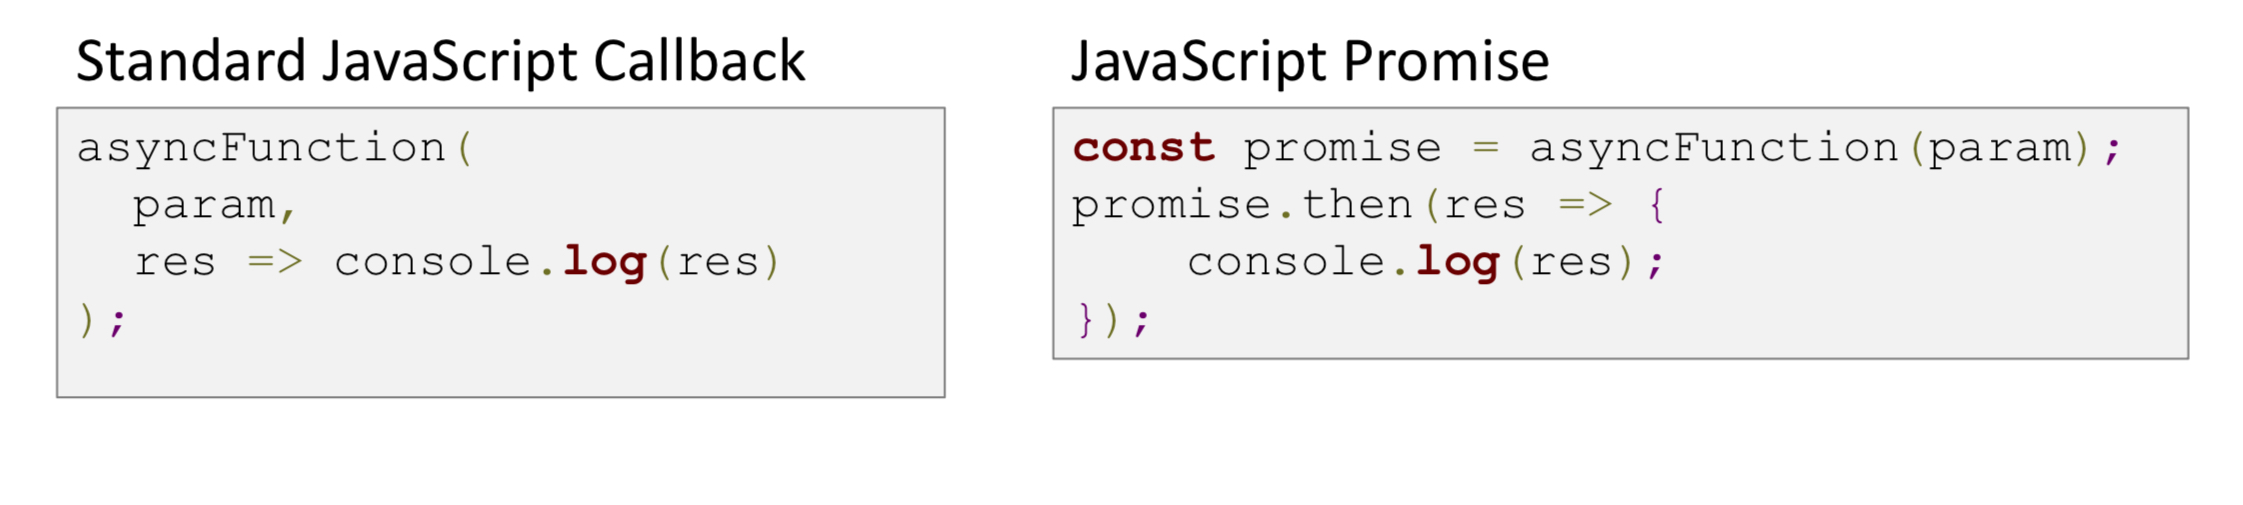
\includegraphics[width=10cm]{async.png}

\section*{React.js}
An open source JavaScript web application framework written in JavaScript, maintained by Meta. It allows you to declare dynamic views in web apps. Applications are cross browser compliant and you can start a React app by running: 
\begin{tcolorbox}
\begin{verbatim}
npx create-react-app <app-name>
\end{verbatim}
\end{tcolorbox}

Features of React include \textbf{Components} which are stateful HTML elements that can be passed as parameters, where state can be used for conditional rendering of components. Relevantly, we will be using \textbf{functional components} rather than older \textbf{class components}. Also, note that there is unidirectional data flow in React as data is passed from parent components to children, and never the reverse. \textbf{JSX} or JavaScript XML is extended JavaScript that allows HTML to be written directly in React components. Further, the \textbf{Virtual DOM} is a view of the HTML tree maintained by React, used to keep track of changes and only re-render components that have changed. Lastly, \textbf{Events}, as in user/system events can trigger callback functions that interact with a given component.

The entire React application starts at a `root' component. Components contain JSX with HTML, or more nested components. Note that, all components are eventually compiled to HTML. Functional components, the preferred type of components, define a component by specifying a function that takes in properties (props) as input and returns JSX as output. Every time a component is rendered, the function is called and JSX is returned. To persist state across renders, the useState() hook is used where useState takes in an initial value and returns the current state and a modifier. To update state, the modifier must be used, which triggers a re-render. Keep in mind that components are rendered lazily -- renders may be batched and not happen immediately -- and changes to state may not be immediately reflected in the state variable until the next render. 

\section*{Node.js} Node.js is an open-source server-side JavaScript runtime environment. \textbf{NPM} or node package manager is a JavaScript package manager. Project dependencies are specified in a file called `package.json' and these dependencies may include \textbf{express} which is a minimalist web server framework, \textbf{mysql} which is a mySQL driver for Node.js, and \textbf{mocha} which is a JavaScript testing framework.

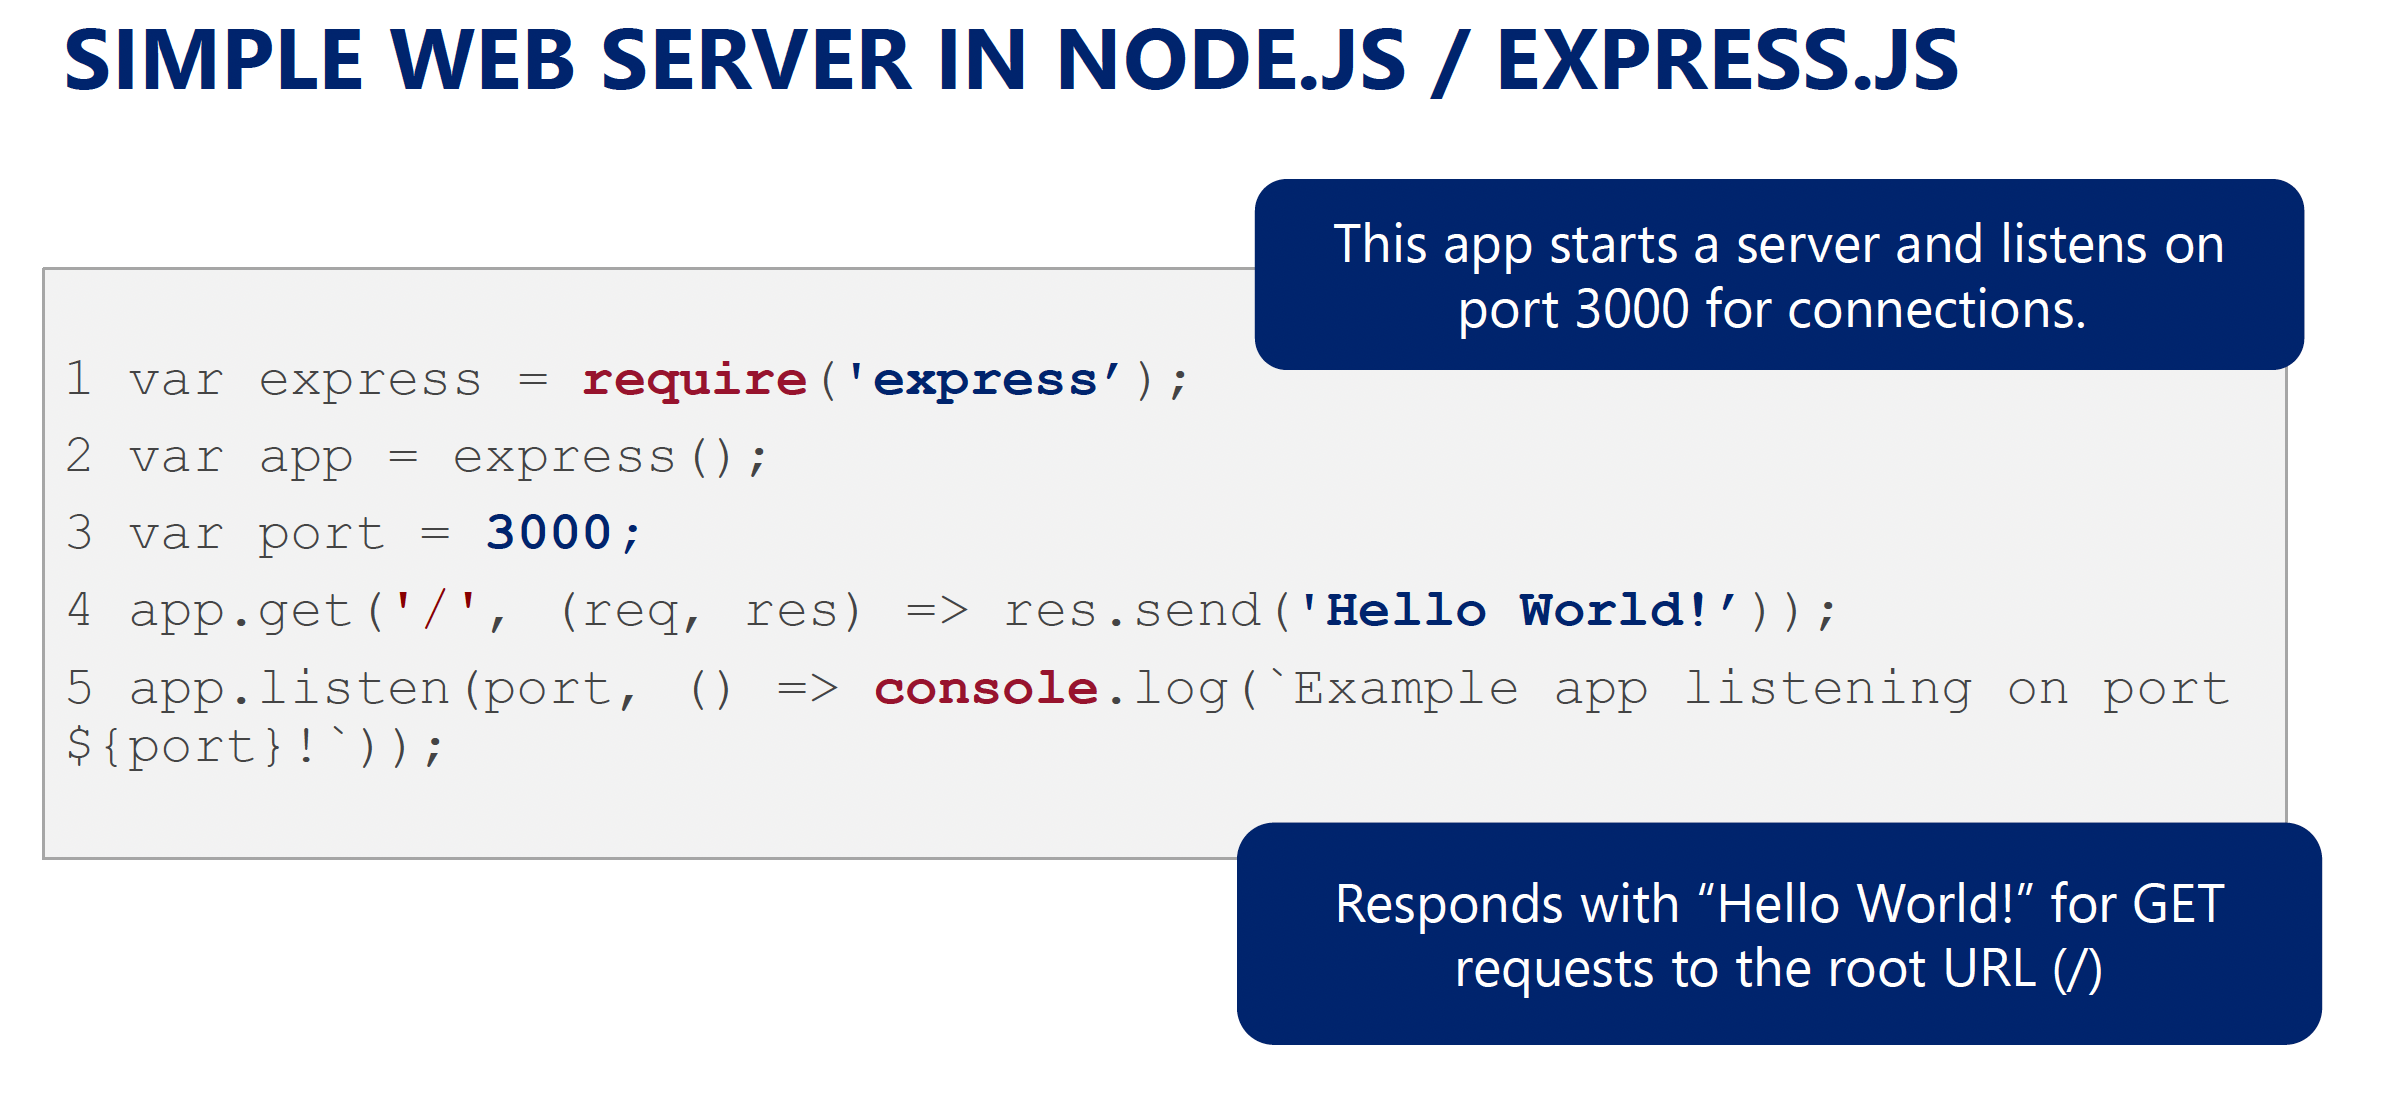
\includegraphics[width=10cm]{webserver.png}

\textbf{Routing} refers to determining how an application responds to a client request to a particular endpoint, which is a URI (or path) and a specific HTTP request method (GET, POST, etc.). Routes have the following structure: \textbf{app.METHOD(PATH, HANDLER)} where app is the instance of Express, METHOD is one of the HTTP request methods, PATH is a path on the server, and HANDLER is a function to be executed when the route is matched. An actual example of this would be:

\begin{tcolorbox}
    \begin{verbatim}
app.get(`/', (req, res) => res.send(`Hello World!'));
    \end{verbatim}
\end{tcolorbox}

\textbf{Parameterized Routes} are named URL segments that are used to capture the values specified at their position in the URL. So, for instance, changing the route URL from `/cart' to `/cart/:uid', will make the given uid value available inside the code as the variable req.params.uid.
\end{document}
